%!TEX root = ../template.tex
%%%%%%%%%%%%%%%%%%%%%%%%%%%%%%%%%%%%%%%%%%%%%%%%%%%%%%%%%%%%%%%%%%%%
%% chapter4_C_PC.tex
%% NOVA thesis document file
%%
%% Chapter with the Hardware Design of the Control, Peripherals&Communications part
%%%%%%%%%%%%%%%%%%%%%%%%%%%%%%%%%%%%%%%%%%%%%%%%%%%%%%%%%%%%%%%%%%%%

\typeout{NT FILE chapter4_C_PC.tex}

\chapter{Hardware Design -- Control, Peripherals and Communications}\label{cha:chapter4_C_PC}

%Meter aqui um pequena introdução do que e mostrado neste capitulo e descrição de seccoes

%SSSSSSSSSSSSSSSSSSSSSSSSSSSSSSSSSSSSSSSSSSSSSSSSSSSSSSSSSSSSSSSSSSSSSSSSSSSS
\section{Control, Peripherals, and Communications}\label{sec:41_C_PC}

Fed by the carefully laid out system's power supply, this chapter focuses on describing the hardware design process of the Control, Peripherals and Communications subgroups of the new architecture, which depend on each other in order to interpret the positioning correction data flow. These subgroups are highlighted in Figure~\ref{fig:architecture_new_C_PC}.

% meter aqui o NOVO diagrama de blocos com C_PC highlight -- INACABADO;
\begin{figure}[h]
	\centering
	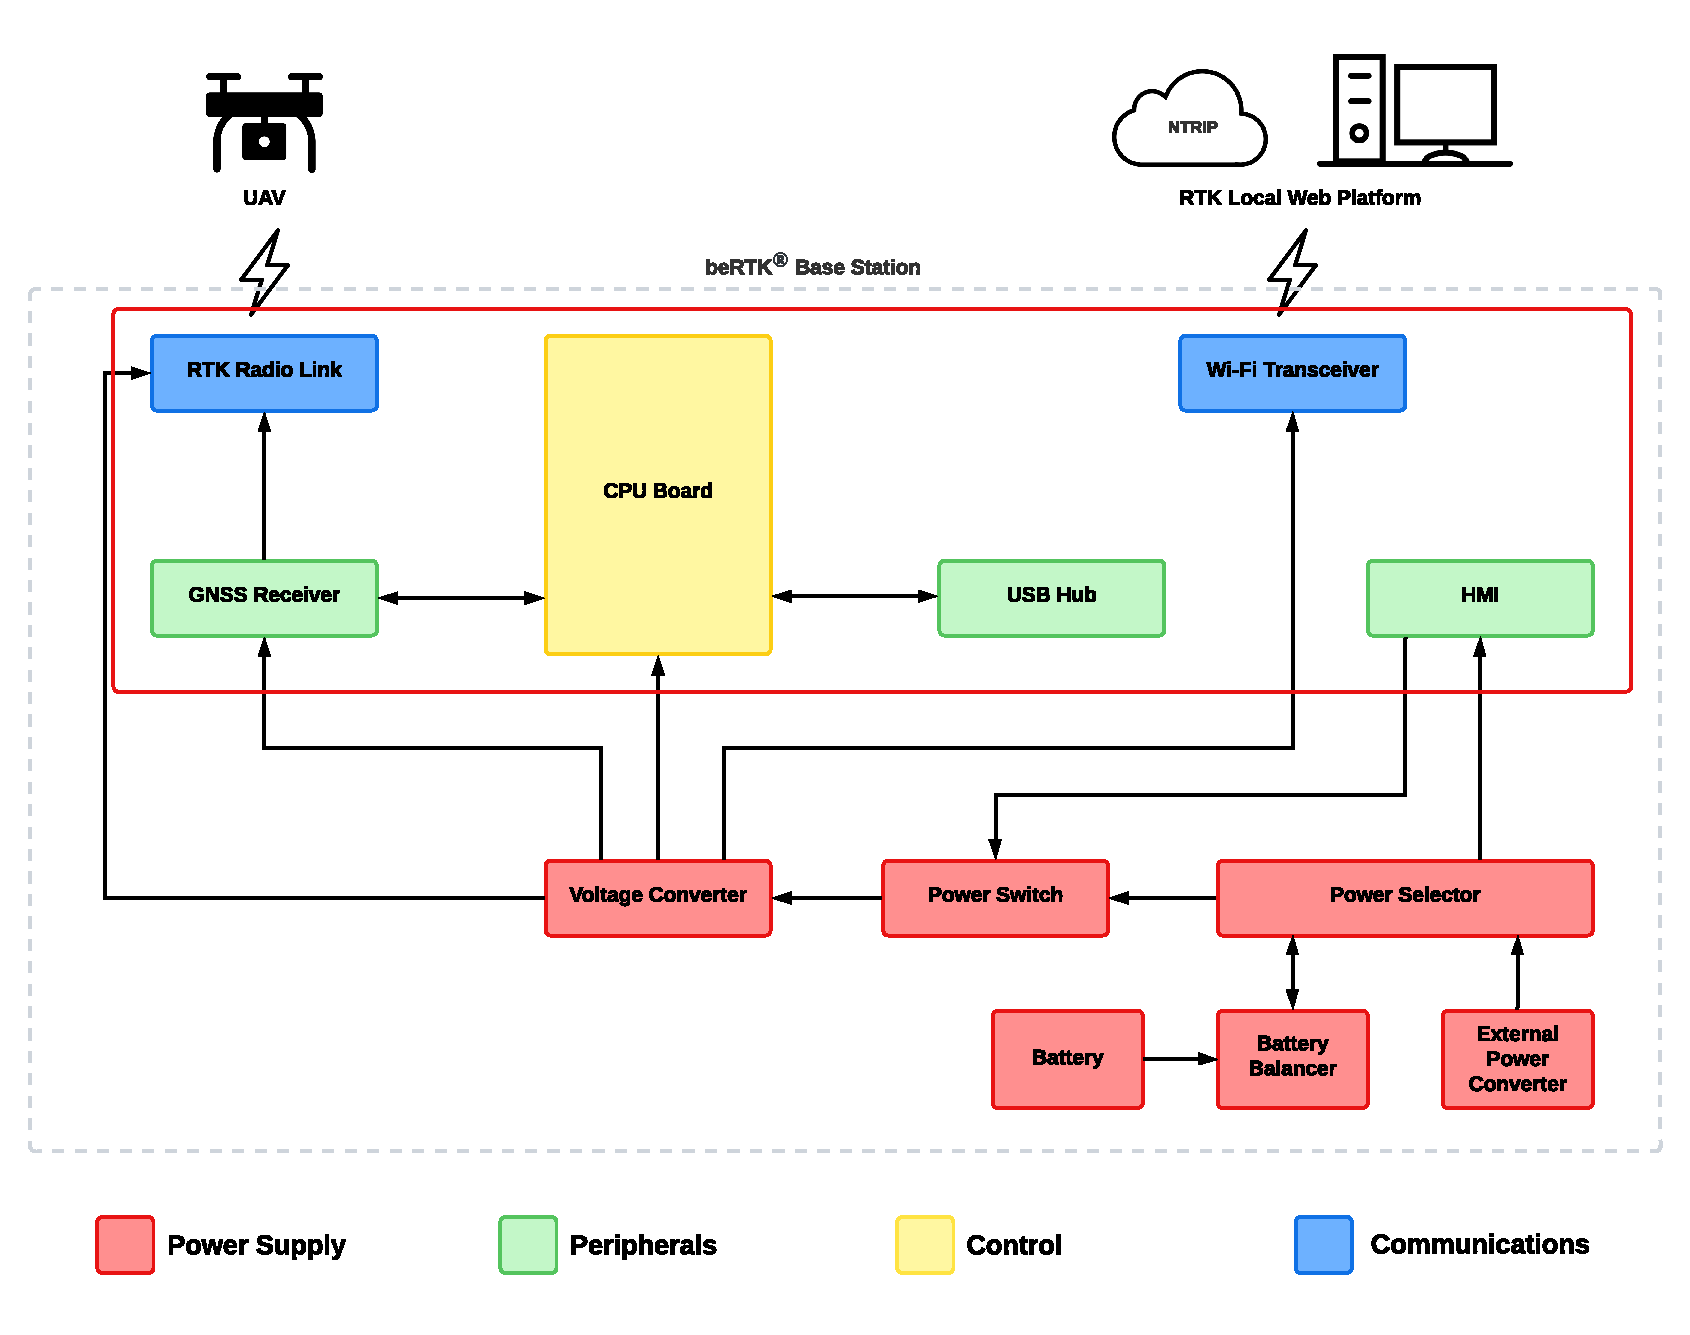
\includegraphics[width=1.0\textwidth]{Chapters/Figures/chapter3/Chapter4_bloackDiagram.pdf}
	\caption{beRTK\textsuperscript{\textregistered}'s new system architecture blocks covered in this chapter.}
	\label{fig:architecture_new_C_PC}
\end{figure}

%sSsSsSsSsSsSsSsSsSsSsSsSsSsSsSsSsSsSsSsSsSsSsSsSsSsSsSsSsSsSsSsSsSsSsSsSsSsS
\section{Control}\label{sec:311_Control}

Starting from the control subgroup, the only component to be selected was a single-board computer able to replace the previously used Raspberry Pi 4 Model B; this means the chosen device would have to be able to carry out a pre-determined set of instructions crucial for the operation of the base station. Such requirement is presented in Section~\ref{sec:II_FCT_requirements} -- requirement \textbf{RTKBS.MAIN.FCT.030}, which proposes the use of a single-board computer (SBC).
The set of instructions performed by the original beRTK\textsuperscript{\textregistered} base station is carried out by a Raspberry Pi 4 Model B computer (described in Section~\ref{sec:II_architecture_Control}), therefore, an element with a comparable computational power as this computer would be ideal. The Raspberry Pi Foundation offers a variety of solutions for many project ideas\footnote[13]{The Raspberry Pi Foundation's hardware offers are available at \url{https://www.raspberrypi.com/products/}.}, and since the operations intended for the beRTK\textsuperscript{\textregistered} base station are so well performed by the Raspberry Pi 4 Model B, it would be worth looking through the array of Raspberry Pi products in order to find a good solution. Research leads to the Raspberry Pi Compute Module 4.
This compact module not only has a small form factor when compared with the Raspberry Pi 4 Model B, but it also bears its computational power, thanks to the same processor (a Broadcom BCM2711 quad-core Cortex-A72 (ARM v8) 64-bit SoC @ 1.5GHz). This makes it a great option for the system's control unit~\cite{CM4}.

%meter imagem CM4:
\begin{figure}[h]
	\centering
	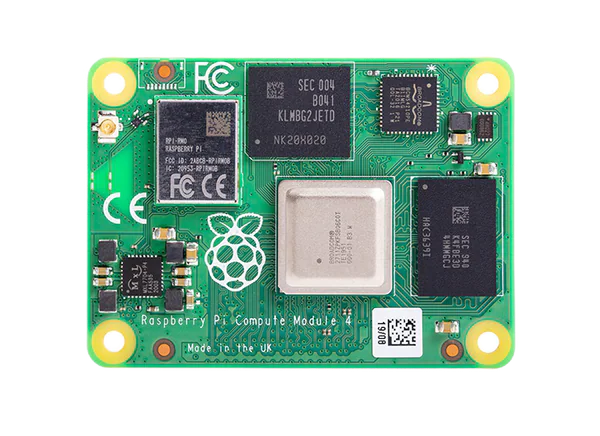
\includegraphics[width=0.5\textwidth]{Chapters/Figures/CM4.png}
	\caption{The Raspberry Pi Compute Module 4 (CM4)~\cite{CM4}.}
	\label{fig:CM4}
\end{figure}

One can choose from thirty-two CM4 variants which differ from each other on RAM and eMMC flash, as well as with or without wireless capabilities.

%sSsSsSsSsSsSsSsSsSsSsSsSsSsSsSsSsSsSsSsSsSsSsSsSsSsSsSsSsSsSsSsSsSsSsSsSsSsS
\section{Peripherals and Communications}\label{sec:312_Peripherals_Communications}

Since this module is intended to be an embedded solution without any of the external ports present in the Raspberry Pi 4 Model B, the relevant ones must be included in the proposed solution, which in this case are USB and HDMI. The CM4 provides all the necessary pins for the implementation of two HDMI connectors on its carrier board (in this case the base station's motherboard); however, when it comes to using its USB interface, the user must add a USB hub, since only two USB data pins are provided, along with a USB On-The-Go (OTG) pin. The latter, is used in order to define the CM4 as either a host or a slave~\cite{CM4}.

%meter imagem do HUB usb: LAN9514

In order to enable such data transfers, the base station requires a way to allow the setup of both upstream and downstream USB ports. The Raspberry Pi 3 Model B uses a chip known as LAN9514, which is a four-port USB 2.0 hub and Ethernet controller. Since this chip has the needed characteristics for the setup of the CM4's USB interface, it was chosen as the main module concerning USB data transfer.

The datasheet for LAN9514 details the IC as a 10/100 Ethernet controller, as well as a USB 2.0 hub with four downstream ports and one upstream port, and targets it for desktop computers and embedded systems, among other uses~\cite{LAN9514}. The LAN9514 also fits the Peripherals subgroup, along with the ZED-F9P module and the HMI, the latter of which bridges the user-device gap via a simple on/off button, LED indicators for both battery status and power source indication and a single connector intended for an external power source, satisfying requirement \textbf{RTKBS.MAIN.PWS.050}, as well as all the requirements defined in Section~\ref{sec:II_HMI_requirements}.

It is also worth mentioning that, referring to requirements \textbf{RTKBS.MAIN.FCT.020} and \textbf{RTKBS.MAIN.FCT.040}, which correspond to the GNSS module (ZED-F9P) and the Wi-Fi transceiver (Digi XBee 3 RF module), respectively, there were no changes in such elements for the new beRTK\textsuperscript{\textregistered}'s proposed solution.

%sSsSsSsSsSsSsSsSsSsSsSsSsSsSsSsSsSsSsSsSsSsSsSsSsSsSsSsSsSsSsSsSsSsSsSsSsSsS

\section{Circuit Design}\label{sec:32_Circuit}

%meter uma pequena introduçao a dizer que usei o kicad e que segui uma metodologia qualquer

%sSsSsSsSsSsSsSsSsSsSsSsSsSsSsSsSsSsSsSsSsSsSsSsSsSsSsSsSsSsSsSsSsSsSsSsSsSsS

\subsection{Control Unit}\label{sec:322_CONTROL}
	%mini introdução
The CM4 \gls{SoM} introduced in Section~\ref{sec:311_Control} is a powerful addition to the new beRTK\textsuperscript{\textregistered}, given its ability of carrying out all the necessary operations required by the system, thanks to the on-board processor, memory and eMMC Flash~\cite{CM4}.

The new beRTK\textsuperscript{\textregistered}'s system will make use of three of the available interfaces offered by the CM4: USB 2.0 (high-speed), HDMI 2.0 and GPIO.

The CM4's electrical interface is made up of two 100-pin high-density connectors, and is powered by the AP64501's 5V supply through the interconnected pins 77, 79, 81, 83, 85 and 87 (visible on the right side of the schematic symbol for the first CM4 connector, MOD1A in Figure~\ref{fig:CM4_GPIO_circuit}).

From a macroscopic point of view, the use of specific interfaces is entrusted with each connector: one is in charge of establishing connections to the high-speed serial interfaces, while the other with the remaining interfaces (among other setup pins), the most important of which is the GPIO.
\cite{CM4} references the BCM2711 ARM peripherals book (\cite{BCM2711_book}), a guide describing all the features provided by the CM4, along with all the alternative functions available, suitable for most designs.

As an important note, it must be mentioned that the Raspberry Pi Foundation provides a development board for the CM4 -- the CM4IO Board\footnote[14]{Available at \url{https://www.raspberrypi.com/products/compute-module-4-io-board/}.} --, whose design intends to allow the testing and understanding of every interface provided by the CM4 module. The design files for this board are also available online, since the Foundation made them fully open source.

%s--Ss--Ss--Ss--Ss--Ss--Ss--Ss--Ss--Ss--Ss--Ss--Ss--Ss--Ss--Ss--Ss--Ss--Ss--S

\subsubsection{High-Speed Serial Interfaces}\label{sec:3221_CM4_HSpeed}

\paragraph{HDMI 2.0 Interface}	Two HDMI 2.0 interfaces are available to use with the CM4 and each have the ability of providing 4K images. For the new beRTK\textsuperscript{\textregistered}, only one HDMI interface is necessary, and therefore only one HDMI port is needed. Figure~\ref{fig:CM4_HighSpeed_circuit} represents the schematic diagram of the second 100-pin connector of the CM4 (MOD1B, with pins 101 to 200), responsible for the high-speed serial interfaces -- two of which are HDMI 2.0. The interface used for the project is labeled as HDMI0, and is represented by every pin connected to an external label that starts with ``HDMI0'' -- 12 pins in total. To the right of the same figure, the HDMI type-A connector port can be seen, represented by F6. To minimize incoming noise from the 5V power supply (i.e. from the AP64501), implemented right before this connector's power input pin is a ferrite bead (FB1) rated at 2.0A, a more-than-sufficient current rating for the project's 5V power supply.

\paragraph{USB 2.0 Interface}	The CM4's USB 2.0 interface enables a signalling rate of 480Mbit/s and is accessible via two pins, USB2\_N and USB2\_P, which represent the negative (D-) and positive (D+) data pins, respectively. In Figure~\ref{fig:CM4_HighSpeed_circuit}, these pins are, in the same order as mentioned, represented by pins 103 and 105; they are connected to the pins $\overline{\mbox{USBDM0}}$ and USBDP0 (pins number 58 and 59, respectively) of the LAN9514 USB 2.0 hub, covered in Section~\ref{sec:3234_LAN9514}.

There is one extra pin (numbered 101) used in this interface, labelled as USB\_OTG\_ID. This pin  provides the CM4's USB port the ability of being used as a true On-The-Go (OTG) port, accomplished by (typically) tying the USB\_OTG\_ID pin to the ID pin of a Micro USB connector. This feature allows the CM4 to act interchangeably as either a host or a device. For this version of the project, there is no necessity of the OTG feature, and as such, the USB\_OTG\_ID pin is simply tied to GND, as that ensures the module will be used as either a fixed host or fixed device, according to~\cite{CM4}.

% meter aqui circuito do CM4_HighSpeed
\begin{figure}[h]
	\centering
	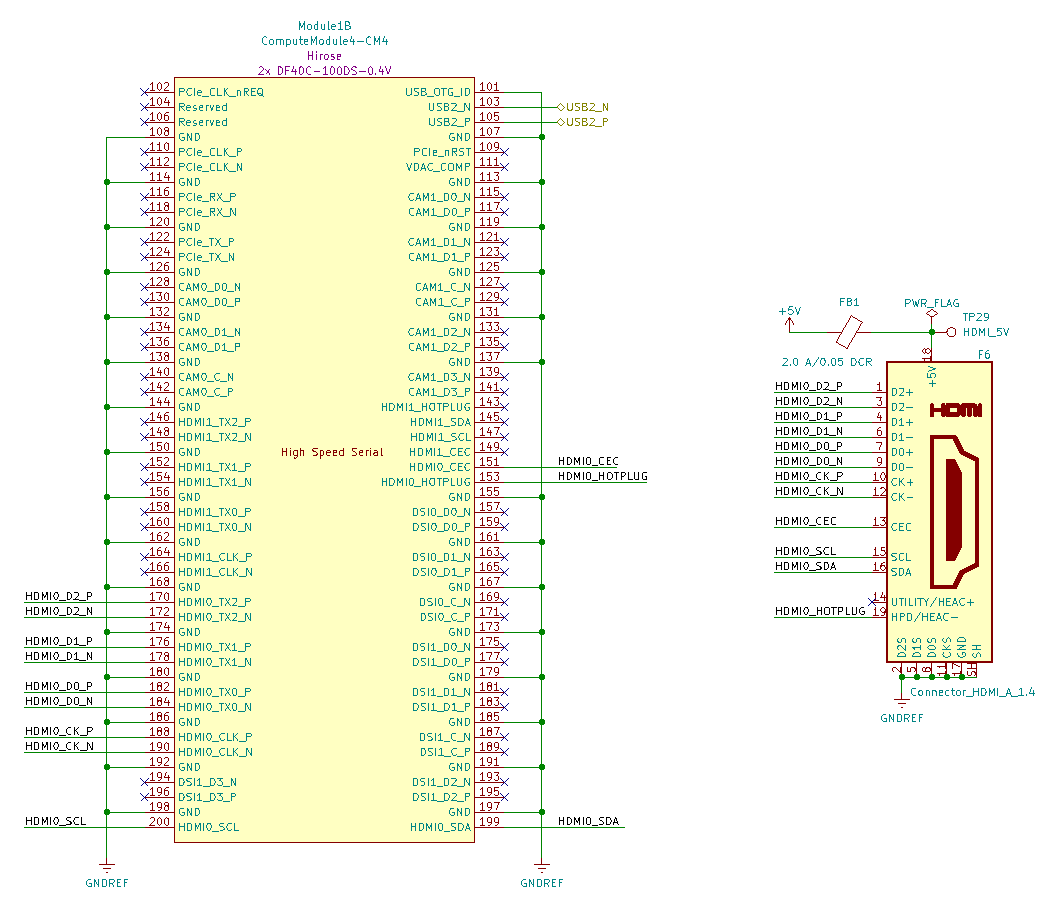
\includegraphics[width=1.0\textwidth]{Chapters/Figures/chapter3/CM4_HighSpeed.pdf}
	\caption{beRTK\textsuperscript{\textregistered} base station's CM4 High Speed schematic diagram.}
	\label{fig:CM4_HighSpeed_circuit}
\end{figure}

% REFERÊNCIA needed!!!!!!!!!!!!!!!!!!!!
%sSsSsSsSsSsSsSsSsSsSsSsSsSsSsSsSsSsSsSsSsSsSsSsSsSsSsSsSsSsSsSsSsSsSsSsSsSsS

\subsubsection{GPIO Interface}\label{sec:3222_CM4_GPIO}

The BCM2711 provides 58 GPIO lines which are split into three different banks. Bank 0 contains all GPIO pins from 0 to 27 -- the only bank used by the CM4. Therefore, the module's GPIO is made up of 28 pins. It is located on the first 100-pin connector of the CM4 (MOD1A, which covers pins 1 to 100) -- represented in Figure~\ref{fig:CM4_GPIO_circuit}. Since the CM4's design is ``loosely based'' on the Raspberry Pi 4 Model B's (\cite{CM4}), the GPIO pins of the former correspond to the same GPIO pins of the latter, and grant access to internal peripherals, such as SMI, DPI, I2C, PWM, SPI, and UART.

The CM4 provides a specially dedicated pin to power bank 0 (and thus set the ``pull'' level to each GPIO pin), labelled GPIO\_VREF (pin 78 in Figure~\ref{fig:CM4_GPIO_circuit}), which can either be tied to the CM4's +1.8V or +3.3V supply output (pins 88 and 90, or pins 84 and 86, respectively). For this project, GPIO\_VREF is tied to the +3.3V pins.

Similarly to the 5V power supply, the +3.3V supply is marked in the schematics of the project by an arrow symbol with a ``+3V3'' label near it, and is hereby referred to as ``3V3''. This net is also used to supply other ICs and components on the beRTK\textsuperscript{\textregistered} system. It must be noted that the load connected to it must not surpass 600mA. As for the total load of the 28 GPIO pins, it should be kept below 50mA.

Besides the ability of standard GPIO operation, all the GPIO pins are able to carry out up to six alternative functions, which can be selected by modifying the address of a corresponding ``Function Select Register'', assigned to each pin. According to~\cite{BCM2711}, for the GPIO pins used in this project -- GPIO4, GPIO8 and GPIO9 (pins 54, 39 and 40, respectively, in Figure~\ref{fig:CM4_GPIO_circuit}) --, the Function Select Register is GPFSEL0. The alternative functions of the GPIO pins used in the project (as well as the ones with test points only\footnote[15]{See Section~\ref{sec:3223_CM4_CTRL_POINTS}.}) are presented in Table~\ref{tab:GPIO_alternative_functions}.

%table GPIO_alternative_functions:
\begingroup
\begin{table}[h]
	\caption{Alternative function assignment of the GPIO pins used in the project (adapted from~\cite{CM4}).}
	\label{tab:GPIO_alternative_functions}
	\centering
	\resizebox{\textwidth}{!}{%
	\begin{tabular}{lccccccc}
        \toprule
        \textbf{GPIO} & \textbf{Pull} & \textbf{ALT0} & \textbf{ALT1} & \textbf{ALT2} & \textbf{ALT3} & \textbf{ALT4} & \textbf{ALT5} \\
        \midrule
        GPIO4 & High & GPCLK0 & SA1 & DPI\_D0 & SPI4\_CE0\_N & TXD3 & SDA3 \\
		\midrule
        GPIO8 & High & SPI0\_CE0\_N & SD0 & DPI\_D4 & BSCSL / CE\_N & TXD4 & SDA4 \\
		\midrule
		GPIO9 & Low & SPI0\_MISO & SD1 & DPI\_D5 & BSCSL / MISO & RXD4 & SCL4 \\
		\midrule
        GPIO12 & Low & PWM0\_0 & SD4 & DPI\_D8 & SPI5\_CE0\_N & TXD5 & SDA5 \\
		\midrule
        GPIO13 & Low & PWM0\_1 & SD5 & DPI\_D9 & SPI5\_MISO & RXD5 & SCL5 \\
		\midrule
        GPIO18 & Low & PCM\_CLK & SD10 & DPI\_D14 & SPI6\_CE0\_N & SPI1\_CE0\_N & PWM0\_0 \\
		\midrule
        GPIO19 & Low & PCM\_FS & SD11 & DPI\_D15 & SPI6\_MISO & SPI1\_MISO & PWM0\_1 \\
		\midrule
        GPIO20 & Low & PCM\_DIN & SD12 & DPI\_D16 & SPI6\_MOSI & SPI1\_MOSI & GPCLK0 \\
		\midrule
        GPIO21 & Low & PCM\_DOUT & SD13 & DPI\_D17 & SPI6\_SCLK & SPI1\_SCLK & GPCLK1 \\
        \bottomrule
    \end{tabular}}
\end{table}
\endgroup

% meter aqui circuito do CM4_GPIO
\begin{figure}[h]
	\centering
	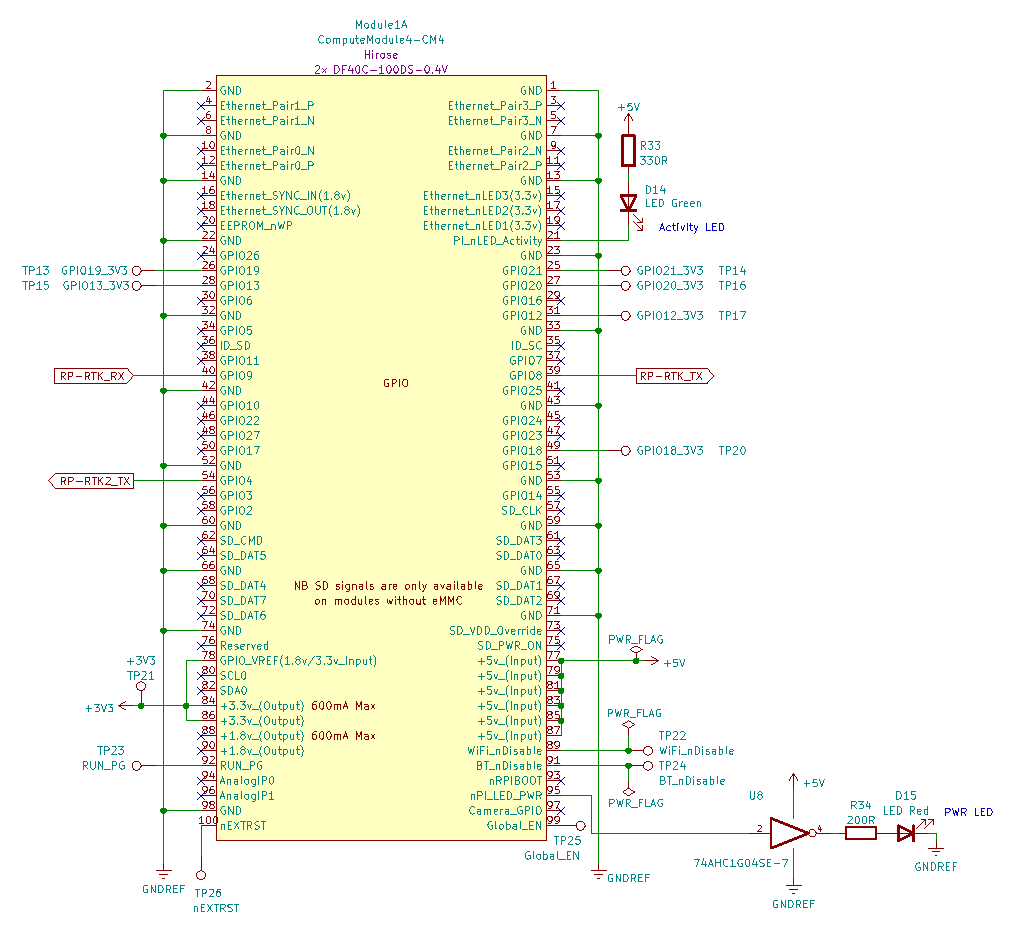
\includegraphics[width=1.0\textwidth]{Chapters/Figures/chapter3/CM4_GPIO.pdf}
	\caption{beRTK\textsuperscript{\textregistered} base station's CM4 GPIO schematic diagram.}
	\label{fig:CM4_GPIO_circuit}
\end{figure}

% REFERÊNCIA needed!!!!!!!!!!!!!!!!!!!!
%s--Ss--Ss--Ss--Ss--Ss--Ss--Ss--Ss--Ss--Ss--Ss--Ss--Ss--Ss--Ss--Ss--Ss--Ss--S

\subsubsection{Status Control Points}\label{sec:3223_CM4_CTRL_POINTS}

\paragraph{Power and Activity LEDs}	To indicate correct power-on, boot and operation of the module, two important pins are available on the CM4 -- the power and activity LED pins:

\begin{itemize}
	\item Pin 95, PI\_LED\_nPWR -- An active-low output used to drive an power-on LED indicator.
	\cite{CM4} informs that the signal output from this pin must be buffered, and together with its active-low topology, the circuit of Figure~\ref{fig:PI_LED_nPWR} can be connected to it.
	%sub-circuito PI_LED_nPWR:
	\begin{figure}[H]
		\centering
		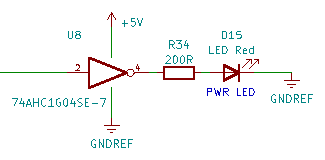
\includegraphics[width=0.6\textwidth]{Chapters/Figures/chapter3/PI_LED_nPWR.pdf}
		\caption{Inverting buffer circuit for the CM4's power-on LED.}
		\label{fig:PI_LED_nPWR}
	\end{figure}
	This small circuit forces the pin's output signal through a 74AHC1G04 single inverter gate, which draws its supply voltage from the AP64501's 5V supply net. Therefore, when fed a low input signal, the output of this inverter will simply correspond to its operating voltage, i.e. 5V. Finally, connecting a reasonably-valued resistor in series with an LED to the inverter's output results in the power-on indicator;

	\item Pin 21, PI\_nLED\_Activity -- With an LED pulled up to 5V, this active-low pin is used to indicate activity of the CM4. It also aids in boot troubleshooting, since it will cause the connected LED to flash in pre-defined patterns that can be decoded using a specialized look-up table\footnote[16]{Available at \url{https://www.raspberrypi.com/documentation/computers/configuration.html}.}.
\end{itemize}

\paragraph{Additional Test Points}	A few test points were added to the design, in order to monitor and debug the CM4's operation.
Also keeping in mind that there is always room for improvement, these test points' utility doubles, in the sense that adding them to the pins of unused interfaces of the module provide valuable status information that can be used to account for future versions of the beRTK\textsuperscript{\textregistered}.
Observing once again Figure~\ref{fig:CM4_GPIO_circuit}, the test points added are:
\begin{itemize}
	\item Pin 99, Global\_EN -- Upon powering on the CM4, this input is internally pulled up to 5V through a 100k$\Omega$ resistor. In case this pin is pulled low, the module is set to its lowest possible power consumption state. Conversely, driving it low (i.e. directly to GND) shuts down the CM4;
	
	\item Pin 100, nEXTRST -- This output is driven high (i.e. to 3V3) once the CM4 starts its booting process. On the other hand, upon reset, the pin will read a logical low voltage, as it becomes tied to the internal GND of the CM4;
	
	\item Pin 92, RUN\_PG -- A bidirectional pin used to signal the run state of the CM4. When on, it is internally pulled up to 3V3 and means the module is running; pulling it low through a resistor (e.g. 220$\Omega$) will reset the module's CPU;

	\item Pin 89, WL\_nDisable -- The CM4 modules can benefit from the addition of an on-board wireless module that supports 2.4 GHz, 5.0 GHz IEEE 802.11 b/g/n/ac wireless, as well as Bluetooth 5.0, BLE. In that case, the WL\_nDisable pin can be used for monitoring the state of the wireless networking. If the voltage on this pin reads a logical high (3.3V), it implies that the wireless module is powered up. Conversely, when this pin is tied or even driven low, the wireless module will not power up (useful for reducing power consumption in designs that do not require wireless features);

	\item Pin 91, BT\_nDisable -- Similarly to pin 89, this pin derives from the same wireless module, and it is used for monitoring the state of Bluetooth on the module. If the voltage on this pin reads a logical high (3.3V), it implies that Bluetooth is powered up. Conversely, when this pin is tied or even driven low, the wireless module will not power up and therefore no Bluetooth features will be available;
	
	\item Pin 31, GPIO12 -- GPIO pin with six alternative functions (see Table~\ref{tab:GPIO_alternative_functions} for more details);

	\item Pin 28, GPIO13 -- GPIO pin with six alternative functions (see Table~\ref{tab:GPIO_alternative_functions} for more details);

	\item Pin 49, GPIO18 -- GPIO pin with six alternative functions (see Table~\ref{tab:GPIO_alternative_functions} for more details);

	\item Pin 26, GPIO19 -- GPIO pin with six alternative functions (see Table~\ref{tab:GPIO_alternative_functions} for more details);

	\item Pin 27, GPIO20 -- GPIO pin with six alternative functions (see Table~\ref{tab:GPIO_alternative_functions} for more details);

	\item Pin 25, GPIO21 -- GPIO pin with six alternative functions (see Table~\ref{tab:GPIO_alternative_functions} for more details).
\end{itemize}

% REFERÊNCIA needed!!!!!!!!!!!!!!!!!!!!
%s--Ss--Ss--Ss--Ss--Ss--Ss--Ss--Ss--Ss--Ss--Ss--Ss--Ss--Ss--Ss--Ss--Ss--Ss--S

\subsection{Peripherals and Communications}\label{sec:323_PERIPHERALS_COMMS}
	%mini introdução

%s--Ss--Ss--Ss--Ss--Ss--Ss--Ss--Ss--Ss--Ss--Ss--Ss--Ss--Ss--Ss--Ss--Ss--Ss--S

\subsubsection{Human-Machine Interface (HMI)}\label{sec:3231_BACKPANEL}

As previously mentioned in Section~\ref{sec:3212_BQ29209}, the battery pack's status voltage (present on the VBAT\_STAT net) is the power supply for IC U6 (Figure~\ref{fig:HMI_circuit}), a low-power quad voltage comparator named LM2901 (by STMicroelectronics~\cite{LM2901}). This voltage comparator is designed to compare four voltage levels with 2.048V, the voltage set by LM404DBZ-2.0 (U7), a precision voltage reference manufactured by Texas Instruments. Since the four internal comparators of the LM2901 are non-inverting, the voltage reference will be tied directly to the negative terminals (xIN-) of the comparators, while the different voltage levels of the battery pack (set by resistors R24, R29, R30, R31 and R32) will be connected to the positive terminals (xIN+). Regarding the LM2901's four outputs (xOUT), in order to achieve the objective of LED voltage status indication (through LEDs D9-D12), each of these is pulled up to 5V through a 330$\Omega$ resistor, in order to drive each LED, in case the respective internal comparator senses the battery's voltage to be higher than the 2.048V reference.

% meter aqui circuito do BACKPANEL
\begin{figure}[h]
	\centering
	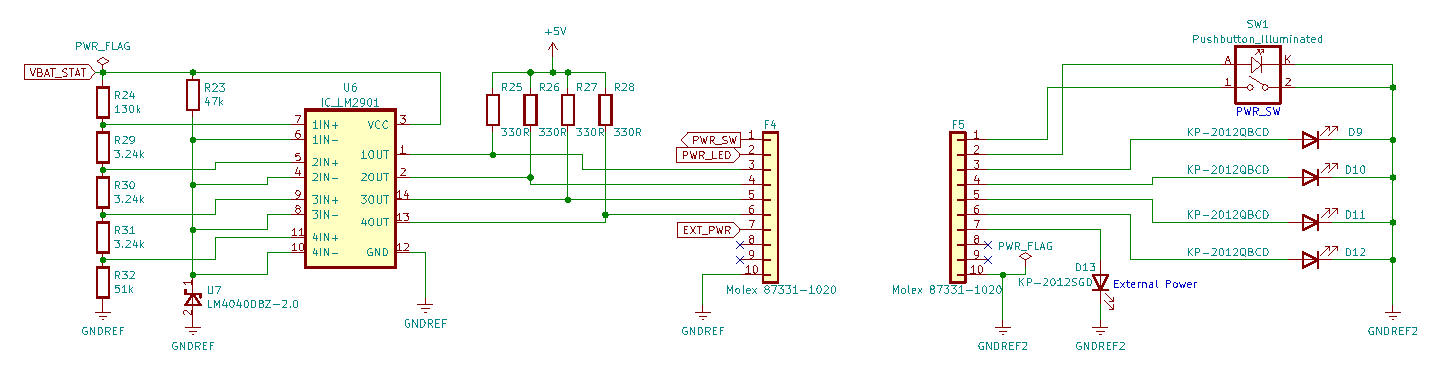
\includegraphics[width=1.0\textwidth]{Chapters/Figures/chapter3/Back_Panel.pdf}
	\caption{beRTK\textsuperscript{\textregistered} base station's HMI schematic diagram.}
	\label{fig:HMI_circuit}
\end{figure}

With this, besides the four battery status indicator LEDs, the system's HMI itself is also composed of the push-button mentioned in Section~\ref{sec:3213_SWITCH} -- used for turning on and of the supply for the AP64501 buck converter --, as well as another LED used to indicate when an external adapter is plugged in and powering the system (D13 in Figure~\ref{fig:HMI_circuit}).

It is considered good practice to include a voltage regulator for the input coming from an external adapter net. For this project, a voltage regulator circuit of this type was implemented, and it is connected to input DCIN of the LTC4012, near the top of Figure~\ref{fig:LTC4012_circuit}. Figure~\ref{fig:EXT_PWR} showcases such a circuit. This circuit is also used to supply power to LED D13, the external power indicator.

% meter aqui circuito do EXT_PWR
\begin{figure}[h]
	\centering
	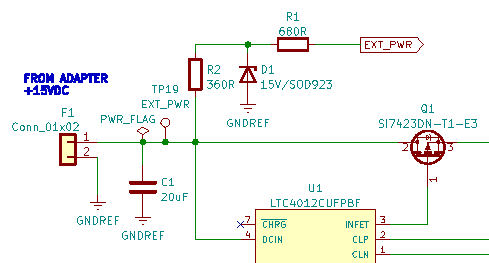
\includegraphics[width=0.6\textwidth]{Chapters/Figures/chapter3/EXT_PWR.pdf}
	\caption{beRTK\textsuperscript{\textregistered} base station's external power voltage reference schematic diagram.}
	\label{fig:EXT_PWR}
\end{figure}

% meter aqui circuito do EXT_PWR
\begin{figure}[h]
	\centering
	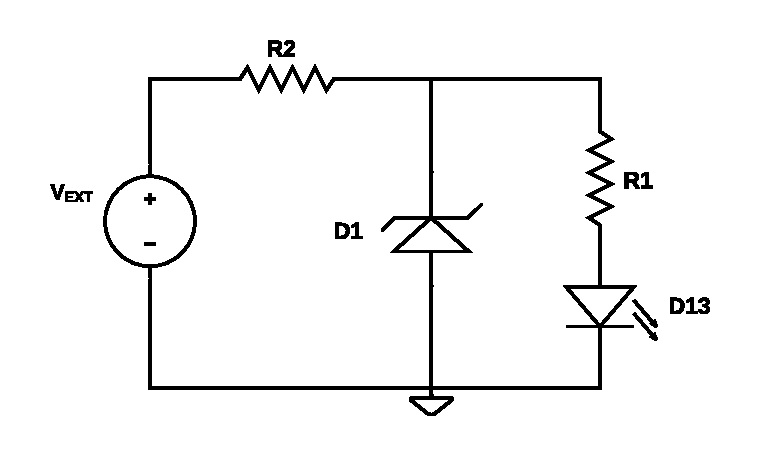
\includegraphics[width=0.6\textwidth]{Chapters/Figures/chapter3/EXT_PWR_2.pdf}
	\caption{beRTK\textsuperscript{\textregistered} base station's external power voltage reference equivalent circuit.}
	\label{fig:EXT_PWR_2}
\end{figure}

It is common to use a Zener diode to build a voltage reference, which was the case for this project. The circuit of Figure~\ref{fig:EXT_PWR} can be approximated by the equivalent circuit of Figure~\ref{fig:EXT_PWR_2}, where $V_{EXT}$ represents the external adapter's input voltage that ranges from +15VDC to +22VDC.

To correctly pick out Zener diode D1, the two most important specifications of this component must be known, which are the Zener voltage ($V_{Z_{D1}}$) and the maximum power dissipation ($P_{Z_{D1}}$). Since the typical DC input voltage for the system was already established at 15V, the criteria was to choose a Zener diode with $V_{Z_{D1}}=15$V. At the time of the project's hardware design phase, the CDZVT2R15B Zener diode model was chosen as the main component of the voltage reference circuit. This model has minimum and maximum Zener voltage values of 14.340V and 14.980V, respectively.
This value can be rounded up to meet the 15V input of the external adapter.
It also bears a maximum power dissipation of 100mW, and therefore $P_{Z_{D1}}=100$mW~\cite{CDZVT2R15B}. This means the maximum current that may flow through D1 ($I_{Z_{D1}}$) is given by expression (\ref{eq:Zener_Imax}):

\begin{equation}\label{eq:Zener_Imax}
	I_{Z_{D1}}=\frac{P_{Z_{D1}}}{V_{Z_{D1}}}=\frac{0.1}{15} \approx 6.667 \textrm{mA}\,\medskip
\end{equation}

The LED model to be used for D13 (visible in Figure~\ref{fig:HMI_circuit}) was already known: KP-2012SGD by Kingbright. This LED presents a typical forward voltage ($V_F$) of 2.2V, and assuming a forward current ($I_F$) of 20mA, Figure~\ref{fig:HMI_circuit} R1's value can be calculated through (\ref{eq:R1_Zener}):

\begin{equation}\label{eq:R1_Zener}
	R1=\frac{V_{Z_{D1}} - V_F}{I_F}=\frac{15 - 2.2}{0.02}=640\Omega \,\medskip
\end{equation}

The nearest standard value for R1 is $634 \Omega$, which causes $I_F$ to be 20.158mA (therefore, $I_{R1}=20.158$mA) -- acceptable as it is lower than the the D13 LED's forward current maximum rating.

Lastly, to determine resistor R2's value, since it is known from Kirchhoff's current law that the current flowing through this component ($I_{R2}$) is equal to the sum of the Zener current and R1's current, i.e. $I_{R2}=I_{Z_{D1}}+I_{R1} \approx 26.825$mA, R2's value can be derived from equation (\ref{eq:R2_Zener}):

\begin{equation}\label{eq:R2_Zener}
	R2 = \frac{V_{EXT_{max}} - V_{Z_{D1}}}{I_{R2}} = \frac{22 - 15}{0.026825} \approx 260.951 \Omega \,\medskip
\end{equation}

The nearest standard value for R2 is $261 \Omega$. In the conditions presented for equation (\ref{eq:R2_Zener}), this results on a flow of 20.153mA on LED D13, which is still completely acceptable.

It must be noted that the LM2901's outputs, as well as nets PWR\_SWITCH, PWR\_LED and EXT\_PWR, which are complementary to the HMI, are connected to the HMI itself (i.e. the push-button SW1 and the power indication LEDs) through two 2.54mm pitch pin headers (F4 and F5 in Figure~\ref{fig:HMI_circuit}), in order to allocate it on a specific user-accessible location of the beRTK\textsuperscript{\textregistered} casing.

% REFERÊNCIA needed!!!!!!!!!!!!!!!!!!!!
%s--Ss--Ss--Ss--Ss--Ss--Ss--Ss--Ss--Ss--Ss--Ss--Ss--Ss--Ss--Ss--Ss--Ss--Ss--S

\subsubsection{GNSS Receiver and RTK Radio Link}\label{sec:3232_ZEDF9P}

The element that provides the system with its distinct GNSS and RTK specifications is also a part of the Peripherals and Communications group. This element is known, as previously mentioned, as ZED-F9P, and it is a high precision module equipped with a multiband GNSS receiver. Therefore, this module can be used in applications that require precise positioning, such as in the agricultural or industrial settings, robotic guidance or, the case study for this project, survey and mapping for UAVs. For that, the module offers centimetre-level accuracy through the use of RTK, which is the main positioning technology adopted for the beRTK\textsuperscript{\textregistered} base station.

% 1º: descrever o simbolo da carrier board:
The implementation the ZED-F9P in the new beRTK\textsuperscript{\textregistered}'s system is achieved through the assembly (to the motherboard) of a secondary board which carries the GNSS module along with external circuitry (i.e. a carrier board) to aid on its use -- particularly, an SMA connector for an antenna to establish the RTK radio link. Beyond Vision has developed this carrier board for an earlier project, and it resulted in the schematic symbol block MOD2, used to represent the system's GNSS module (Figure~\ref{fig:ZEDF9P_circuit}).

	% meter aqui circuito do ZEDF9P
\begin{figure}[h]
	\centering
	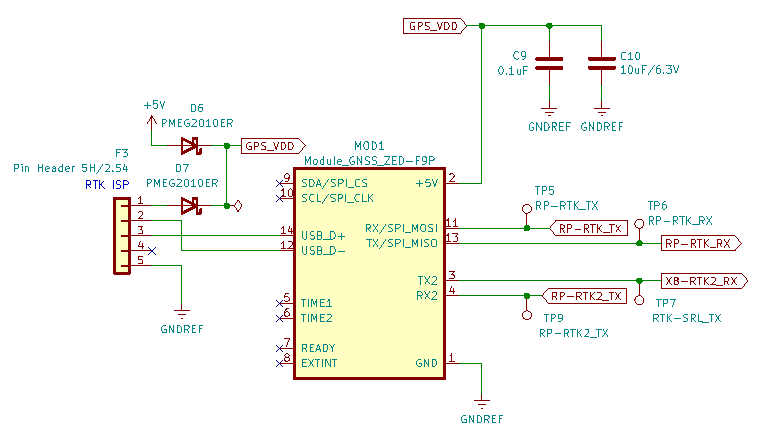
\includegraphics[width=1.0\textwidth]{Chapters/Figures/chapter3/Modules_ZEDF9P.pdf}
	\caption{beRTK\textsuperscript{\textregistered} base station's GNSS module schematic diagram.}
	\label{fig:ZEDF9P_circuit}
\end{figure}

% 2º: como aparece o símbolo no projeto da base station --  esse será o simbolo ao qual vou SEMPRE fazer referência:
Analysing the circuit of Figure~\ref{fig:ZEDF9P_circuit}, with the help of ZED-F9P's datasheet (\cite{ZED_F9P}), it can be verified that the pins used on this GNSS module correspond to the following ZED-F9P pins:
\begin{itemize}
	\item Pin 3, TX2 -- Corresponds to pin 27 on the ZED-F9P module. This pin is used as an UART correction output. Connected to pin 4 of the Wi-Fi transceiver (Figure~\ref{fig:XBEE3_circuit});

	\item Pin 4, RX2 -- Corresponds to pin 26 on the ZED-F9P module. This pin is used as an UART correction input. Connected to the GPIO4 pin of the CM4 (Figure~\ref{fig:CM4_GPIO_circuit});
 
	\item Pin 13, TX/SPI\_MISO -- Corresponds to pin 42 on the ZED-F9P module. Depending of the logical state of a dedicated interface selector input named D\_SEL, this pin can be used as either a host UART output (if D\_SEL high or open) or SPI\_MISO (if D\_SEL low). Connected to the GPIO9 pin of the CM4 (Figure~\ref{fig:CM4_GPIO_circuit});

	\item Pin 11, RX/SPI\_MOSI -- Corresponds to pin 43 on the ZED-F9P module. Depending of the logical state of a dedicated interface selector input named D\_SEL, this pin can be used as either a host UART input (if D\_SEL high or open) or SPI\_MOSI (if D\_SEL low). Connected to the GPIO8 pin of the CM4 (Figure~\ref{fig:CM4_GPIO_circuit});

	\item Pin 14, USB\_D+ -- Corresponds to pin 40 on the ZED-F9P module. This is a bidirectional pin used for USB data transit and is commonly known as the USB ``plus'' data pin;

	\item Pin 12, USB\_D- -- Corresponds to pin 39 on the ZED-F9P module. This is a bidirectional pin used for USB data transit and is commonly known as the USB ``minus'' data pin;
\end{itemize}

Regarding the power pins, it can be seen in Figure~\ref{fig:ZEDF9P_circuit} that pin 1 of MOD2 connects to the GND net and pin 2 to the 5V power supply net output from the AP64501, via a Schottky barrier rectifier (D6) -- PMEG2010ER model~\cite{PMEG2010ER}. This diode is strategically placed amid the 5V net and the power input for the GNSS module (net GPS\_VDD) as a way to protect it from possible problems that may arise from discharges or the high switching rate of the buck converter (input capacitors C9 and C10 also aid in such occasions). As such, the model chosen should have a low forward voltage value, in order to maintain the input power for the GNSS module as close as possible to 5V.

Another Schottky barrier rectifier (D7) is placed between the GPS\_VDD net and pin 1 of connector F3, which corresponds to the power pin of a micro USB connector. With a maximum reverse voltage 20V (\cite{PMEG2010ER}), D7 is placed in such a way that only allows power to flow from the USB connector when it is connected, and not the other way around. This micro USB connector is connected to the GNSS module via the USB data pins of the latter (14 and 12, USB\_D+ and USB\_D-, respectively) and is used to program the ZED-F9P.

%não posso meter esta figura aqui porque nao faz parte do meu projeto.
% \begin{figure}[h]
% 	\centering
% 	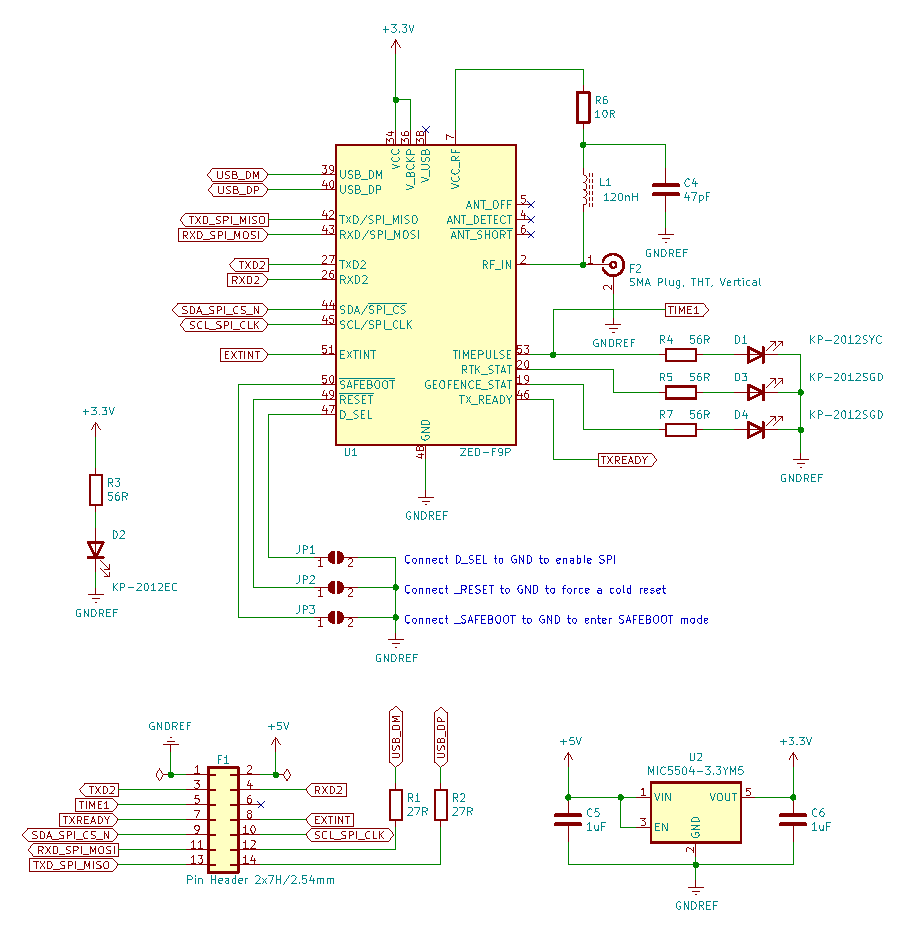
\includegraphics[width=1.0\textwidth]{Chapters/Figures/chapter3/ZED-F9P_carrier_board.pdf}
% 	\caption{Schematic diagram of the carrier board for the ZED-F9P GNSS module, developed by Beyond Vision.}
% 	\label{fig:ZEDF9P_carrier_board}
% \end{figure}

% REFERÊNCIA needed!!!!!!!!!!!!!!!!!!!!
%s--Ss--Ss--Ss--Ss--Ss--Ss--Ss--Ss--Ss--Ss--Ss--Ss--Ss--Ss--Ss--Ss--Ss--Ss--S

\subsubsection{Wi-Fi Transceiver}\label{sec:3233_XBEE3}

As mentioned in Chapter~\ref{cha:chapter2_SotA}, the XBee 3 RF module is used in the system in order to establish a communication line with an external computer through a Wi-Fi radio link. Figure~\ref{fig:XBEE3_circuit} depicts the circuit implementation of the module in the beRTK\textsuperscript{\textregistered}, represented by schematic block MOD3.

% meter aqui circuito do XBEE3
\begin{figure}[h]
	\centering
	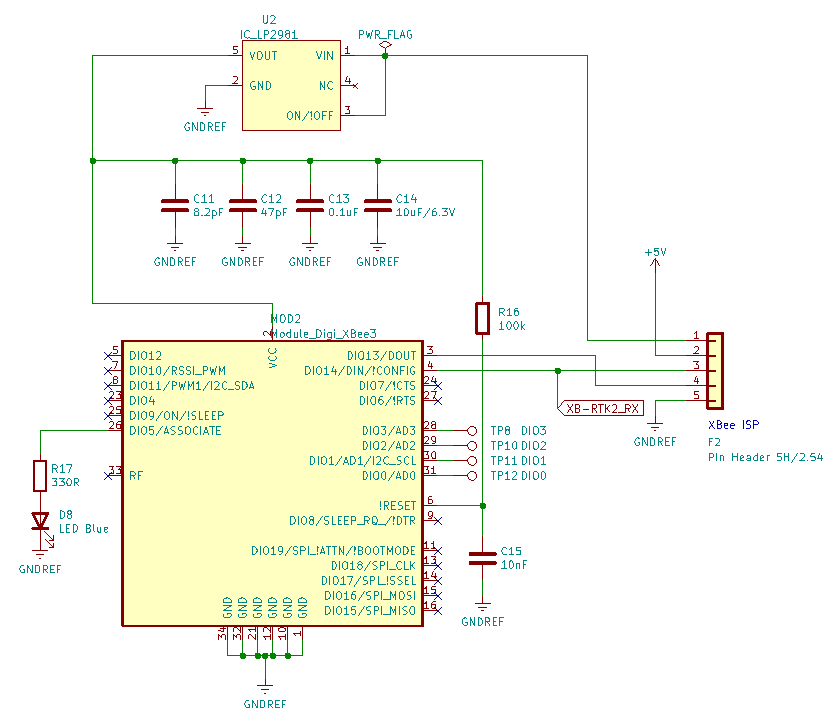
\includegraphics[width=1.0\textwidth]{Chapters/Figures/chapter3/Modules_XBEE3.pdf}
	\caption{beRTK\textsuperscript{\textregistered} base station's Wi-Fi module schematic diagram.}
	\label{fig:XBEE3_circuit}
\end{figure}

Following the module's hardware reference manual (\cite{XBee}), it is recommended that, if only two-way communication is desired from this module, then only pins VCC, GND, DIN and DOUT need to be connected. Pin 4 corresponds to DIO14/DIN/!CONFIG and is, by default, an input pin. It can be defined as either an UART data input or GPIO pin. Setting it up as an UART data input (or an RX pin) and connecting it to pin 3 of the GNSS module (TX2; Figure~\ref{fig:ZEDF9P_circuit}) makes sense, since, as mentioned in Section~\ref{sec:3232_ZEDF9P}, the latter will be defined as an UART output for positioning correction data. Pin 3 corresponds to DIO13/DOUT and is the UART data output counterpart to DIO14/DIN/!CONFIG.

In order to load Zigbee firmware onto the XBee 3 module's hardware and define its pins' functions, connector F2 in Figure~\ref{fig:XBEE3_circuit} is used as an ISP header. This header doubles its functionality, as it also provides power to a regulator, which in turn powers the RF module via the VCC pin. The regulator, named LP2981, is an ultra-low dropout regulator, and its datasheet (\cite{LP2981}) provides a typical application circuit for an LP2981 which, when supplied with 5V by an external regulator (in this case the AP64501), provides a 3.3V output. The design is achieved through the implementation of a total output bypass capacitance ($C_{OUT}$) of no less than $3.3 \mu$F -- which can be increased without limit to improve transient response. Using a different 3.3V power supply just for the XBee is beneficial, since there will be no disturbances from other ICs powered by that source, which would otherwise harm the power signal fed to the vital communication module.

Six other pins of the XBee are also used:
\begin{itemize}
	\item Pin 6, !RESET -- Active-low device reset. Permanently connected to the output terminal of the LP2981 via a 100k$\Omega$ resistor (R16);
 
	\item Pin 31, DIO0/AD0 -- Can be used as either an analog input or GPIO pin, or as an input for a commissioning button to an associate LED;

	\item Pin 30, DIO1/AD1/I2C\_SCL -- Can be used as either an analog input or GPIO pin, or as a serial clock for an I2C communication protocol;

	\item Pin 29, DIO2/AD2 -- Can be used as either an analog input or GPIO pin;

	\item Pin 28, DIO3/AD3 -- Can be used as either an analog or GPIO input;

	\item Pin 26, DIO5/ASSOCIATE -- Can be used as either an associate indicator or GPIO pin.
\end{itemize}

% REFERÊNCIA needed!!!!!!!!!!!!!!!!!!!!
%s--Ss--Ss--Ss--Ss--Ss--Ss--Ss--Ss--Ss--Ss--Ss--Ss--Ss--Ss--Ss--Ss--Ss--Ss--S

\subsubsection{USB 2.0 Hub}\label{sec:3234_LAN9514}

As stated earlier in Section~\ref{sec:312_Peripherals_Communications}, the LAN9514 is an IC that operates as a USB 2.0 hub, while also doubling its functionality as a 10/100 Ethernet controller. Figure~\ref{fig:LAN9514_blockDiagram} from~\cite{LAN9514} details the internal block diagram of the IC. 

%meter imagem LAN9514 block diagram:
\begin{figure}[h]
	\centering
	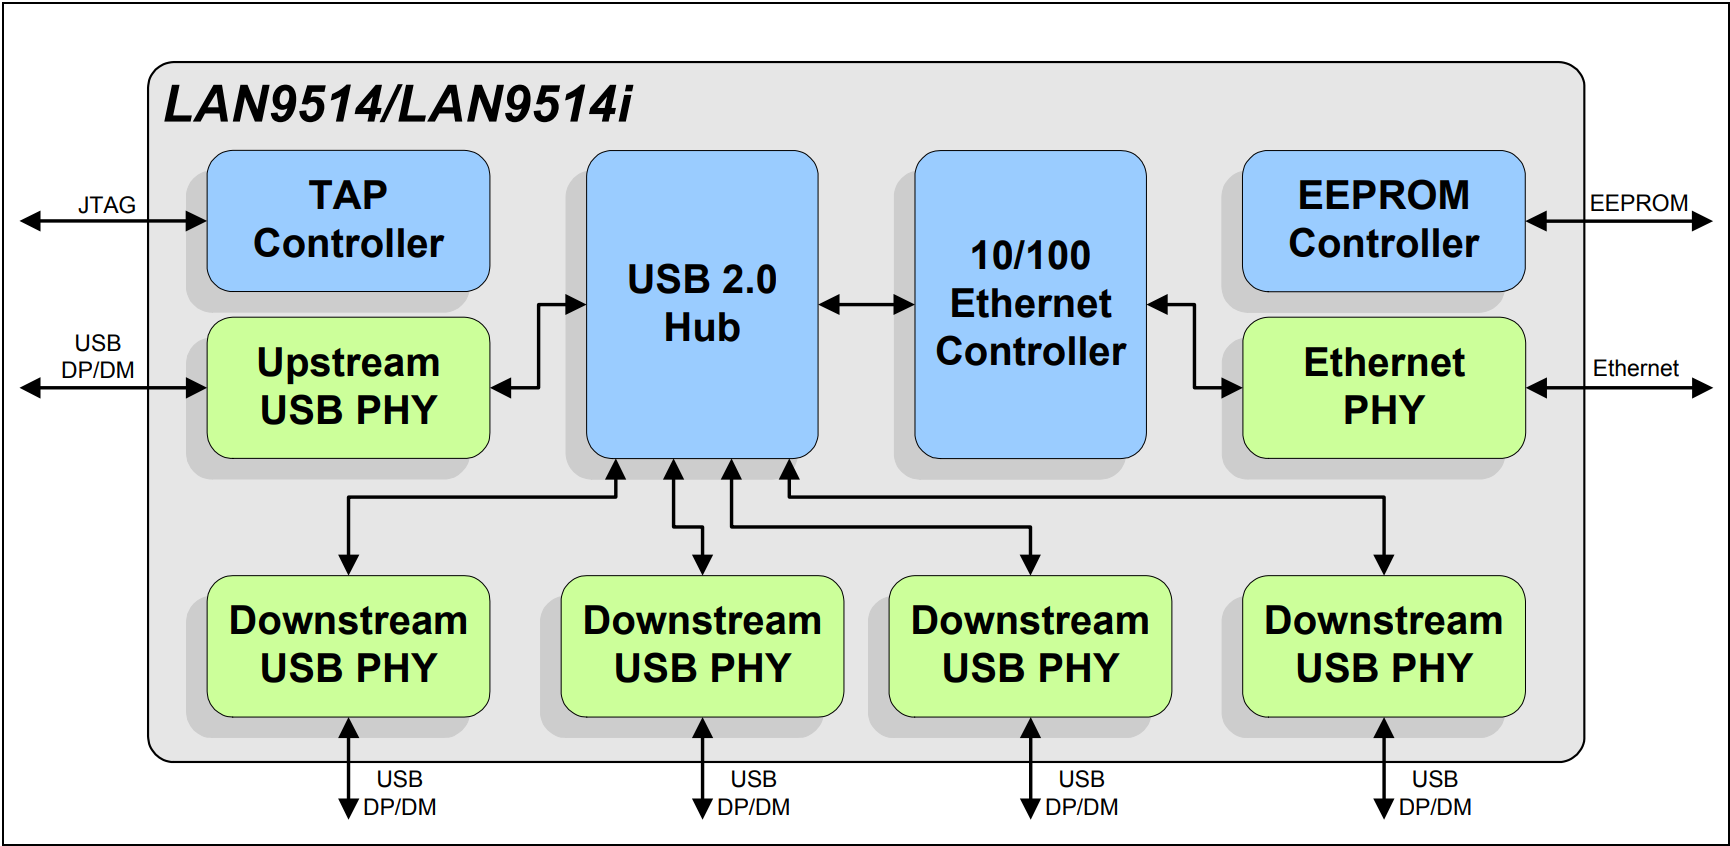
\includegraphics[width=1.0\textwidth]{Chapters/Figures/chapter3/LAN9514_blockDiagram.png}
	\caption{LAN9514/LAN9514i internal block diagram~\cite{LAN9514}.}
	\label{fig:LAN9514_blockDiagram}
\end{figure}

Since for this project only the USB specifications of this IC are needed, the TAP, Ethernet (and its PHY) and EEPROM controllers blocks' implementation was (carefully) left out. The upstream USB PHY block implementation was also left out, although it is required to load the Raspberry Pi operating system (Raspberry Pi OS) into the CM4 module. However, this was not a problem, since the CM4IO board (referenced in the last paragraph of Section~\ref{sec:322_CONTROL}) that provides the user with such possibility was available during the project development stage.

The hub is designed to be fully compliant with the USB 2.0 specification, and is therefore able to comfortably operate with signalling rates of up to 480Mbit/s (i.e. high-speed). This operating mode is particularly interesting to the new beRTK\textsuperscript{\textregistered}'s application, since the CM4 module's USB interface also operates with high-speed signalling rates, as described in Section~\ref{sec:3221_CM4_HSpeed}.

Similarly to the other ICs referenced in this project, a typical application circuit is also available for the LAN9514. This reference design (\cite{LAN9514_ref_schematic}) is divided into seven interdependent circuits that allow engagement with all interfaces of the hub. The schematic of Figure~\ref{fig:USB_Hub_1_circuit} presents the circuit implementation around the LAN9514 itself (represented by U9), adapted from the reference design.%parei aqui - começar desde o numero 1

% meter aqui circuito do USB_Hub_1
\begin{figure}[h]
	\centering
	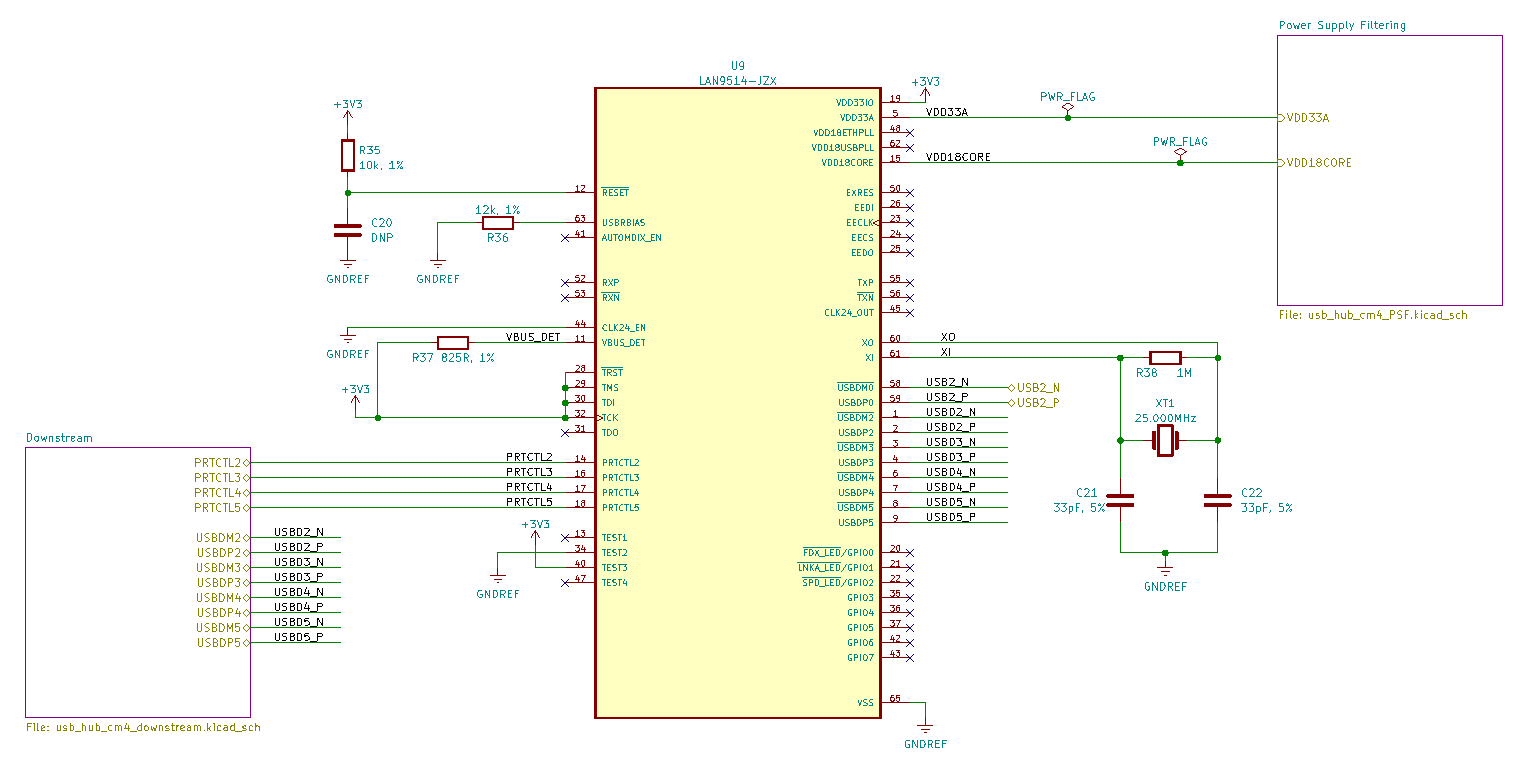
\includegraphics[width=1.0\textwidth]{Chapters/Figures/chapter3/USB_Hub_1.pdf}
	\caption{beRTK\textsuperscript{\textregistered} base station's USB hub schematic diagram.}
	\label{fig:USB_Hub_1_circuit}
\end{figure}

Starting with

% meter aqui circuito do USB_Hub_1 -- POWER SUPPLY FILTERING
\begin{figure}[h]
	\centering
	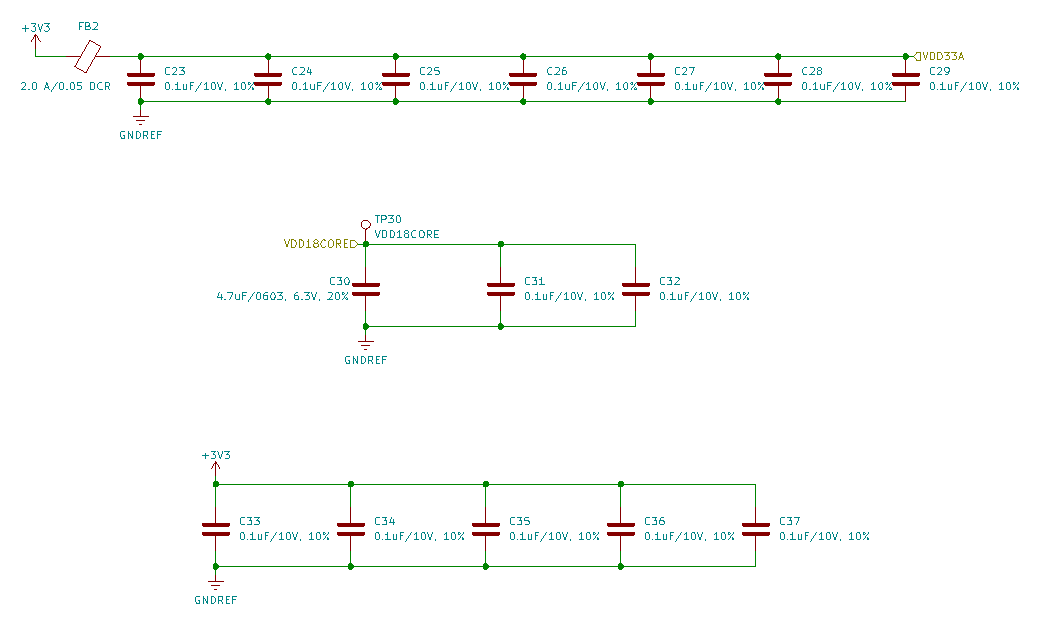
\includegraphics[width=1.0\textwidth]{Chapters/Figures/chapter3/USB_Hub_PwrSplyFiltering.pdf}
	\caption{beRTK\textsuperscript{\textregistered} base station's USB hub Power Supply Filtering schematic diagram.}
	\label{fig:USB_Hub_PwrSplyFiltering_circuit}
\end{figure}

% meter aqui circuito do USB_Hub_1 -- DOWNSTREAM
\begin{figure}[h]
	\centering
	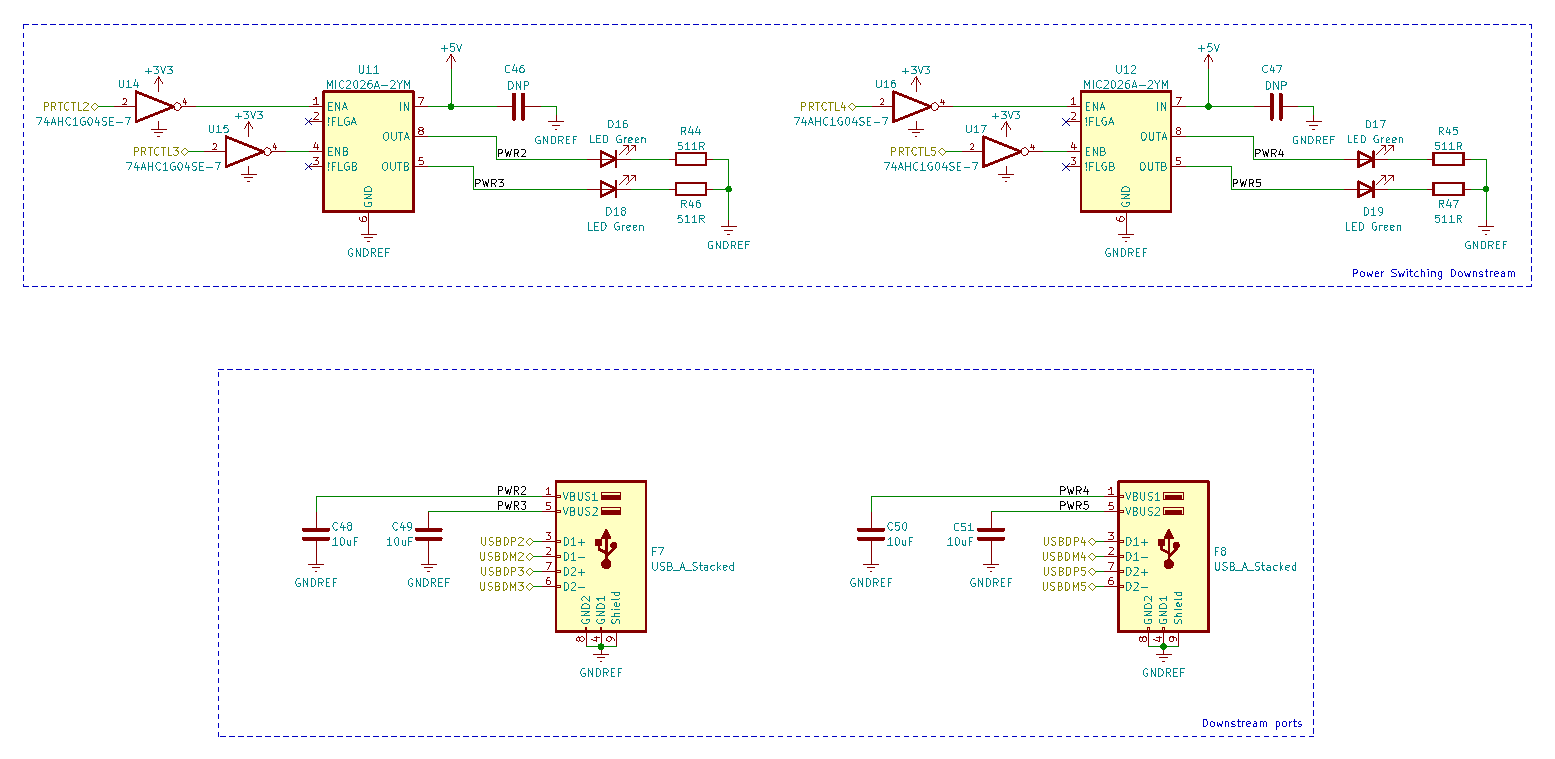
\includegraphics[width=1.0\textwidth]{Chapters/Figures/chapter3/USB_Hub_Downstream.pdf}
	\caption{beRTK\textsuperscript{\textregistered} base station's USB hub Downstream schematic diagram.}
	\label{fig:USB_Hub_Downstream_circuit}
\end{figure}

% REFERÊNCIA needed!!!!!!!!!!!!!!!!!!!!
%SSSSSSSSSSSSSSSSSSSSSSSSSSSSSSSSSSSSSSSSSSSSSSSSSSSSSSSSSSSSSSSSSSSSSSSSSSSS


% \section{PCB Layout Design}\label{sec:33_PCBlayout}

% -- $20 \mu$F ceramic capacitors were chosen for both the power inputs and power output of the LTC4012. 

% -- As mentioned before, the top and bottom power FETs Q2 and Q9, along with inductor L1 are vital to the PWM control architecture. These components are part of the sub-circuit that starts from the +15VDC source of power and passes across FET Q1 (connected to pin INFET), sense resistor R3, 
% This sub-circuit forms the ``power supply rail'', and upon layout design of the circuit from Figure~\ref{fig:LTC4012_circuit}, this section must bear a track width large enough to withstand large values of currents or any other phenomena that may occur (e.g. voltage/current spikes). The needed track width can be calculated through the following expression:

%XBee: Digi XBee 3 RF Module Hardware Reference Manual
% We design XBee 3 RF Modules to be self-sufficient and have minimal sensitivity to nearby processors,
% crystals or other printed circuit board (PCB) components. Keep power and ground traces thicker than
% signal traces and make sure that they are able to comfortably support the maximum current
% specifications. There are no other special PCB design considerations to integrate XBee 3 RF Modules,
% with the exception of antennas.
